% This version of CVPR template is provided by Ming-Ming Cheng.
% Please leave an issue if you found a bug:
% https://github.com/MCG-NKU/CVPR_Template.

% \documentclass[review]{cvpr}
\documentclass[final]{cvpr}

\usepackage{times}
\usepackage{epsfig}
\usepackage{graphicx}
\usepackage{amsmath}
\usepackage{amssymb}

% Include other packages here, before hyperref.

% If you comment hyperref and then uncomment it, you should delete
% egpaper.aux before re-running latex.  (Or just hit 'q' on the first latex
% run, let it finish, and you should be clear).
\usepackage[pagebackref=true,breaklinks=true,colorlinks,bookmarks=false]{hyperref}


\def\cvprPaperID{****} % *** Enter the CVPR Paper ID here
\def\confYear{CVPR 2021}
% \setcounter{page}{4321} % For final version only


\begin{document}

%%%%%%%%% TITLE
\title{Some Interpretation of Transformer Block}

\author{Zichen Tian\\
Nanyang Technological University\\
Singapore\\
{\tt\small ztian002@e.ntu.edu.sg}
}

\maketitle


%%%%%%%%% ABSTRACT
\begin{abstract}
This is a MANUSCRIPT interprets Transformer~\cite{vaswani2017attention}. This work explores the working principle of Transformer and self-attention mechanism theoretically, and tried to clearly answer why they works well. 
\end{abstract}

%%%%%%%%% BODY TEXT
\section{Questions}
% First introduce the outline of transformer. And then go to the details of how every components work. 
This work tried to answer following questions: 
\begin{enumerate}
    \item What is the difference between feed-forward and self-attention, and why this difference ensures self-attention outperforming FF? 
    \item Why call the query the "query"? What's the significance of re-mapping the input $X$ to $Q,K,V$? 
    \item How the dimension $d_K$ of $Q,K\in{\mathbb{R}^{n\times{d_k}}}$ and $d_V$ of $V\in{\mathbb{R}^{n\times{d_v}}}$ affects the training? As long as possible is good.
    \item What's the significance of inner-product in self-attention? Can I replace them to other forms? 
    \item Why normalize the self-attention by factor $\sqrt{d_k}$ in~\cite{vaswani2017attention}?
\end{enumerate}

This work tried to explain the self-attention by modelling the input $(x_i, x_j)$ as two random processing $X_1(t=i), X_2(t=j)$. By this way the self-attention is a representation of cross-correlation $Corr(X_1(i), X_2(j))=E[X_1(i),X_2(j)]\approx\frac{sum}{length}$.
\section{Transformer Block}

\subsection{General Form}
\label{sec:general}
\begin{figure}[ht]
\begin{center}
\fbox{
   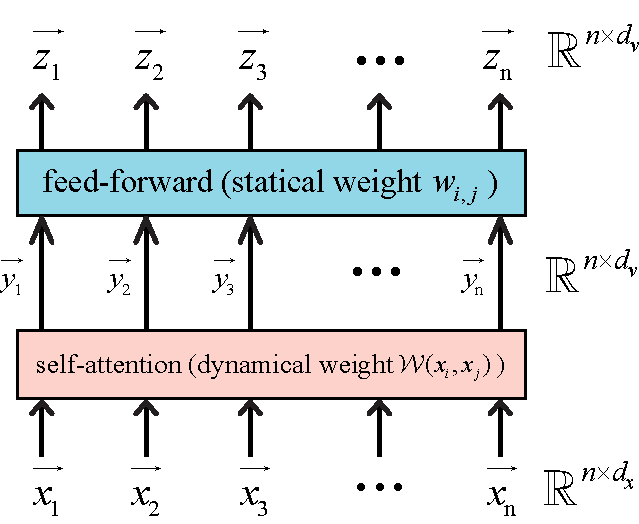
\includegraphics[width=0.9\linewidth]{images/transformer-overall.pdf}
   }
\end{center}
   \caption{Transformer block: self-attention and feed-forward. The residual connection are omitted for clearer view.
   }
\label{fig:transformerover}
\end{figure}

Transformer Block consists of two layers: self-attention and feed-forward layer. Both of them perform the weighted sum on the input, as shown in \autoref{fig:transformerover}.

The input is row vectors $x_i$, in which $i$ is the position of the input, and $d_x$ is the dimension of each input vector. There's totally $n$ positions ($n$ word embeddings).

\begin{align*}
    x_i=[x_i^1, x_i^2, ..., x_i^n]\in\mathbb{R}^{1\times{d_x}}, i\in[1,n]
\end{align*}

Self-attention layer can be modeled generally as \autoref{eq:all-sa}, and feed-forward as \autoref{eq:all-ff}. In \autoref{eq:all-sa}, $y_i$ is the output of self-attention layer, and in \autoref{eq:all-ff} $z_i$ is the output of whole transformer block. the $y_i, z_i\in\mathbb{R}^{1\times{d_v}}$, $i\in[1,n]$. $\mathbb{N}$ is the normalization operation. $\mathcal{W}(x_i,x_j)$ is the self-attention value between input position $i$ and $j$. 

\begin{align}
    {y_i}&=\mathbb{N}\left[\sum_{j}\mathcal{W}(x_i,x_j)\times{v}({x_j})+x_i\right]\label{eq:all-sa}\\
    {z_i}&=\mathbb{N}\left[\sum_jw_{i,j}\times{y_j}+y_i\right]\label{eq:all-ff}
\end{align}

\subsection{Specific Form in Attention Paper}
In \autoref{sec:general}, a general representation of transformer is given. Specifically, by the definition from~\cite{vaswani2017attention}, the $\mathcal{W}(x_i,x_j)=Softmax(\frac{\langle x_iW^q,x_jW^k\rangle}{\sqrt{d_k}})$, and $v(x_j)=x_jW^v$. The $W^q, W^k, W^v$ are weight matrix to be train. $W^q,W^k\in\mathbb{R}^{{d_x}\times{d_k}}$, $W^v\in\mathbb{R}^{d_x\times{d_v}}$.

If define $X=[x_1;x_2;...;x_n]$\footnote{Symbol ; means $X$ is column vector of $x_i$. $X$ is the input matrix containing all positions.}, $Y=[y_1;y_2;...;y_n]$, we have:

\begin{align}
    Y&=\mathbb{N}\left[Softmax\left(\frac{XW^q(XW^k)^T}{\sqrt{d_k}}\right)XW^v+X\right]\\
     &=\mathbb{N}\left[Softmax\left(\frac{XW^q(W^k)^TX^T}{\sqrt{d_k}}\right)XW^v+X\right]
\end{align}

Let $Q=XW^q, K=XW^k, V=XW^v$, than $Q,K\in\mathbb{R}^{n\times{d_k}}$, $V\in\mathbb{R}^{n\times{d_v}}$. We have self-attention layer defined as \autoref{eq:attn}:

\begin{equation}
    Y=\mathbb{N}\left[Softmax\left(\frac{QK^T}{\sqrt{d_k}}\right)V+X\right]\label{eq:attn}
\end{equation}
    

\subsection{Scale-invariant Mapping}
\label{sec:simap}

All the input of self-attention layer are mapped to a higher dimension space\footnote{$Q,K,V$ follow the definition in~\cite{vaswani2017attention}}:

\begin{align}
    Q=XW^q,K=XW^k: \mathbb{R}^{n\times{d_x}}&\to\mathbb{R}^{n\times{d_k}}\\
    V=XW^v: \mathbb{R}^{n\times{d_x}}&\to\mathbb{R}^{n\times{d_v}}
\end{align}

This mapping has two important features:

\begin{enumerate}
    \item Invariant in scale. $X\to Q,K,V$ are scale-invariant mapping, which means for all the vectors $x_i$, the mapping operations are the same, and the relative position between $i$-th vector and $j$-th vector won't change. E.g. $q_1=x_1W^q, q_2=x_2W^q$, with $W^q$ shared, $q_1, q_2$ will follow the same distribution as $x_1, x_2$.
    \item Inherited chain. E.g. $q_i\sim x_i$ and only related with $x_i$. Or in other words, $q_i$ is a direct and exclusive projection of $x_i$. The mapping can be inherited to form a long chain. E.g. given $Q=XW^q, E=QW^e, F=EW^f$, we still have $f_1\sim e_1\sim q_1\sim x_1$.
\end{enumerate}

With above two properties, we can treat $Q,K,V$ as $X$ itself in following analysis.


\subsection{Self-attention}
\label{sec:self-attn}

As proved in \autoref{sec:simap}, mapping $Q=XW^q: \mathbb{R}^{n\times d_x}\to\mathbb{R}^{n\times d_k}$ is a scale-invariant mapping, similar for $V,K$. Thus we could replace $Q,K,V$ with $X$ in \autoref{eq:attn} to see what did self-attention layer does to $X$ directly:

\begin{equation}
    Y\sim \mathbb{N}\left[Softmax\left(\frac{XX^T}{\sqrt{d_k}}\right)X+X\right]
\end{equation}

Knowing $Softmax(\cdot)$, $(\frac{\cdot}{\sqrt{d_k}})$ and $\mathbb{N}[\cdot]$ are statistical operations, we can also remove them to have a clear view to the self-attention:

\begin{equation}
    Y\sim XX^TX+X\footnote{What if $Y\sim Q\times Softmax\left(\frac{K^TV}{\sqrt{d_k}}\right)+X$?}\label{eq:attn-sim}
\end{equation}

\autoref{eq:attn-sim} is a concise model revealing self-attention layer's working principle. Give insights to the intrinsic motivation of this layer.

\subsection{Feed-forward}
\label{sec:ff}

For comparison with self-attention, feed-forward's simplified formula are given in \autoref{eq:ff-sim} (matrix version of \autoref{eq:all-ff}, $W \in \mathbb{R}^{n\times n}$ is a static weight matrix):

\begin{equation}
    Z\sim WY + Y\label{eq:ff-sim}
\end{equation}

Compare \autoref{eq:attn-sim} and \autoref{eq:ff-sim}. They are both weighted sum of input. Only difference is the weight matrix. For self-attention, weight $XX^T=\{\langle\vec{x_i},\vec{x_j}\rangle\}$ is the inner-product between every pair of input positions. While for feed-forward, weight $W=\{w_{i,j}\}$ is a fixed weight.

\textbf{What's the difference between self-attention and feed-forward?}

Meaning of the two weight matrices are different. Because inner-product is a measurement of projection between two vectors, self-attention's weight is a measure of similarity between two input vectors $x_i,, x_j$\footnote{Does similar input vector means the two position have stronger connection?: No}; while for feed-forward, the weight measures the contribution from each input $x_j$ to the output $y_i$.

\section{Further}
\subsection{Scale-invariant Mapping}
\textbf{Is it necessary to re-scale the $d_x$ input to $d_v$ output?}
As shown in TBC, the longer the factor, the more accurate the inner-product could estimate the correlation between two input vectors.

\subsection{Self-attention}
\label{sec:rp}

However, inner-product can not provide a solid measuring of the relationship between two positions, and the normalization parameter $\sqrt{d_k}$ is not reasonable as well. In \autoref{sec:rp}, we will discuss the using of inner-product.

{\small
\bibliographystyle{ieee_fullname}
\bibliography{ref}
}

\end{document}
